\documentclass[]{ltjarticle}
\usepackage[T1]{fontenc}
\usepackage{lmodern}
\usepackage{amssymb,amsmath}
\usepackage{ifxetex,ifluatex}
\usepackage{fixltx2e} % provides \textsubscript
% use upquote if available, for straight quotes in verbatim environments
\IfFileExists{upquote.sty}{\usepackage{upquote}}{}
\ifnum 0\ifxetex 1\fi\ifluatex 1\fi=0 % if pdftex
  \usepackage[utf8]{inputenc}
\else % if luatex or xelatex
  \ifxetex
    \usepackage{mathspec}
    \usepackage{xltxtra,xunicode}
  \else
    \usepackage{fontspec}
  \fi
  \defaultfontfeatures{Mapping=tex-text,Scale=MatchLowercase}
  \newcommand{\euro}{€}
\fi
% use microtype if available
\IfFileExists{microtype.sty}{\usepackage{microtype}}{}
\usepackage{listings}
\usepackage{longtable,booktabs}
\usepackage{graphicx}
% Redefine \includegraphics so that, unless explicit options are
% given, the image width will not exceed the width of the page.
% Images get their normal width if they fit onto the page, but
% are scaled down if they would overflow the margins.
\makeatletter
\def\ScaleIfNeeded{%
  \ifdim\Gin@nat@width>\linewidth
    \linewidth
  \else
    \Gin@nat@width
  \fi
}
\makeatother
\let\Oldincludegraphics\includegraphics
{%
 \catcode`\@=11\relax%
 \gdef\includegraphics{\@ifnextchar[{\Oldincludegraphics}{\Oldincludegraphics[width=\ScaleIfNeeded]}}%
}%
\ifxetex
  \usepackage[setpagesize=false, % page size defined by xetex
              unicode=false, % unicode breaks when used with xetex
              xetex]{hyperref}
\else
  \usepackage[unicode=true]{hyperref}
\fi
\hypersetup{breaklinks=true,
            bookmarks=true,
            pdfauthor={@kohske},
            pdftitle={RマークダウンとPandocで楽々レポート作成},
            colorlinks=true,
            citecolor=blue,
            urlcolor=blue,
            linkcolor=magenta,
            pdfborder={0 0 0}}
\urlstyle{same}  % don't use monospace font for urls
\usepackage[normalem]{ulem}
% avoid problems with \sout in headers with hyperref:
\pdfstringdefDisableCommands{\renewcommand{\sout}{}}
\setlength{\parindent}{0pt}
\setlength{\parskip}{6pt plus 2pt minus 1pt}
\setlength{\emergencystretch}{3em}  % prevent overfull lines
\setcounter{secnumdepth}{5}
\usepackage{xcolor}
\lstset{
  basicstyle=\small\ttfamily, 
  backgroundcolor=\color{gray!9.6},
  columns=[l]{fullflexible} ,
  belowcaptionskip=1.25em,
  frame=single,
  breaklines=true,
  numbers=left
}

\title{RマークダウンとPandocで楽々レポート作成}
\author{@kohske}
\date{2014/3/1}

\begin{document}
\maketitle

{
\hypersetup{linkcolor=black}
\setcounter{tocdepth}{3}
\tableofcontents
}
\section{はじめに}\label{ux306fux3058ux3081ux306b}

Rマークダウンでドキュメントとコード書いて→ knit() → pandoc → (html
\textbar{} pdf \textbar{} docx) します。

\subsection{役に立つ資料}\label{ux5f79ux306bux7acbux3064ux8cc7ux6599}

\begin{itemize}
\itemsep1pt\parskip0pt\parsep0pt
\item
  @teramonagiさんの資料

  \begin{itemize}
  \itemsep1pt\parskip0pt\parsep0pt
  \item
    Tokyo.R@36 ~knitr+pandocではじめる~『R MarkdownでReproducible
    Research』
    \url{http://www.slideshare.net/teramonagi/tokyo-r36-20140222}
  \item
    Tokyo.R@36 ~knitrパッケージではじめる~『R MarkdownでReproducible
    Research』の基礎編のコード
    \url{http://rpubs.com/teramonagi/TokyoR36_Basic}
  \item
    Tokyo.R@36 ~knitrパッケージではじめる~『R MarkdownでReproducible
    Research』の応用編のコード
    \url{http://rpubs.com/teramonagi/TokyoR36_Advanced}
  \end{itemize}
\item
  Pandoc ユーザーズガイド 日本語版
  \url{http://sky-y.github.io/site-pandoc-jp/users-guide/}
\item
  TeX Wiki \url{http://oku.edu.mie-u.ac.jp/~okumura/texwiki/}
\item
  マークダウン用 github.css
  \url{https://gist.github.com/andyferra/2554919}
\end{itemize}

も参考にしてくださいね〜

\section{メタ情報の記述}\label{ux30e1ux30bfux60c5ux5831ux306eux8a18ux8ff0}

マークダウンファイルにはメタ情報を含めることができます。

\subsection{簡易記法}\label{ux7c21ux6613ux8a18ux6cd5}

ファイル先頭を

\begin{lstlisting}
% タイトル
% 著者
% 日付
\end{lstlisting}

で始めることができます。

\subsection{YAML記法}\label{yamlux8a18ux6cd5}

ファイルの先頭にYAMLでメタ情報を入れることができます。次の例を参考にして下さい。

\begin{lstlisting}
---
title: RマークダウンとPandocで楽々レポート作成
author: "@ohske"
tags: [R, pandoc, Dynamic Documentation]
abstract: Rマークダウンでドキュメントとコード書いて→ knit() → pandoc → (html | pdf | docx)します。
---
\end{lstlisting}

\section{レポート生成コマンド
(おなじない)}\label{ux30ecux30ddux30fcux30c8ux751fux6210ux30b3ux30deux30f3ux30c9-ux304aux306aux3058ux306aux3044}

まずは、

\begin{lstlisting}[language=R]
library(knitr)
knit("pandoc-md.Rmd")
\end{lstlisting}

としてRマークダウンファイル(.Rmd)からマークダウンファイルを作成します。
続いて、マークダウンファイルをPandocによって様々な形式に変換します。

\begin{itemize}
\item
  HTMLファイルの作成

\begin{lstlisting}[language=bash]
$ pandoc -s --toc -c github.css --mathjax pandoc-md.md -o pandoc-md.html
\end{lstlisting}

  \begin{itemize}
  \itemsep1pt\parskip0pt\parsep0pt
  \item
    github.cssというファイルを同じフォルダに入れときます。
  \end{itemize}
\item
  LaTeXファイルの作成

\begin{lstlisting}[language=bash]
$ pandoc -s --toc --number-sections --listings -V documentclass=ltjarticle -H preamble.tex pandoc-md.md -o pandoc-md.tex
\end{lstlisting}

  \begin{itemize}
  \itemsep1pt\parskip0pt\parsep0pt
  \item
    必要の応じてプリアンブルを記述したpreamble.texを準備します。
  \end{itemize}
\item
  PDFファイルの作成

\begin{lstlisting}[language=bash]
$ pandoc --toc --number-sections --listings -V documentclass=ltjarticle -H preamble.tex --latex-engine=lualatex -H preamble.tex pandoc-md.md -o pandoc-md.pdf
\end{lstlisting}

  \begin{itemize}
  \itemsep1pt\parskip0pt\parsep0pt
  \item
    必要の応じてプリアンブルを記述したpreamble.texを準備します。
  \end{itemize}
\item
  DOCXファイルの作成

\begin{lstlisting}[language=bash]
$ pandoc pandoc-md.md -o pandoc-md.docx
\end{lstlisting}
\item
  HTML5スライド(slidy)の作成

\begin{lstlisting}[language=bash]
$ pandoc -s --mathjax -i -t slidy pandoc-md.md -o pandoc-slidy.html
\end{lstlisting}
\item
  PDFスライド(Bearer)の作成

\begin{lstlisting}[language=bash]
$ pandoc -t beamer --listings -H preamble-beamer.tex --latex-engine=lualatex pandoc-md.md -o pandoc-beamer.pdf
\end{lstlisting}

  \begin{itemize}
  \itemsep1pt\parskip0pt\parsep0pt
  \item
    必要の応じてプリアンブルを記述したpreamble-beamer.texを準備します。
  \end{itemize}
\end{itemize}

\subsection{R上でpandocを使う}\label{rux4e0aux3067pandocux3092ux4f7fux3046}

knitrパッケージには\lstinline!pandoc()!という関数があるんですが、オプション渡すのが面倒なので\lstinline!system()!でpandocを実行します。

\begin{lstlisting}[language=R]
knit("pandoc-md.Rmd")
system("pandoc -s --toc -c github.css --mathjax pandoc-md.md -o pandoc-md.html")
system("pandoc -s --toc --number-sections --listings -V documentclass=ltjarticle -H preamble.tex pandoc-md.md -o pandoc-md.tex")
system("pandoc --toc --number-sections --listings -V documentclass=ltjarticle --latex-engine=lualatex -H preamble.tex pandoc-md.md -o pandoc-md.pdf")
system("pandoc pandoc-md.md -o pandoc-md.docx")
system("pandoc -s --mathjax -i -t slidy pandoc-md.md -o pandoc-slidy.html")
system("pandoc -t beamer --listings -H preamble-beamer.tex --latex-engine=lualatex pandoc-md.md -o pandoc-beamer.pdf")
\end{lstlisting}

\section{例:あやめの解析
(またかよ・・・orz)}\label{ux4f8bux3042ux3084ux3081ux306eux89e3ux6790-ux307eux305fux304bux3088orz}

\textbf{あやめ}とは、\sout{さかな}植物の名前です。おそらく、世界中でも最も多く解析にさらされた植物でしょう。

学名は\emph{Iris sanguinea}といいます。イリスではなくて、アイリスです。
\textsubscript{大きい声では言えませんが今でも「イリス」と呼んでます。}

\subsection{データの雰囲気}\label{ux30c7ux30fcux30bfux306eux96f0ux56f2ux6c17}

\begin{lstlisting}[language=R]
pander::pandoc(head(iris), caption="あやめのデータ (1-6行)", split.tables = 100)
\end{lstlisting}

\begin{longtable}[c]{@{}ccccc@{}}
\toprule\addlinespace
\begin{minipage}[b]{0.18\columnwidth}\centering
Sepal.Length
\end{minipage} & \begin{minipage}[b]{0.17\columnwidth}\centering
Sepal.Width
\end{minipage} & \begin{minipage}[b]{0.18\columnwidth}\centering
Petal.Length
\end{minipage} & \begin{minipage}[b]{0.17\columnwidth}\centering
Petal.Width
\end{minipage} & \begin{minipage}[b]{0.11\columnwidth}\centering
Species
\end{minipage}
\\\addlinespace
\midrule\endhead
\begin{minipage}[t]{0.18\columnwidth}\centering
5.1
\end{minipage} & \begin{minipage}[t]{0.17\columnwidth}\centering
3.5
\end{minipage} & \begin{minipage}[t]{0.18\columnwidth}\centering
1.4
\end{minipage} & \begin{minipage}[t]{0.17\columnwidth}\centering
0.2
\end{minipage} & \begin{minipage}[t]{0.11\columnwidth}\centering
setosa
\end{minipage}
\\\addlinespace
\begin{minipage}[t]{0.18\columnwidth}\centering
4.9
\end{minipage} & \begin{minipage}[t]{0.17\columnwidth}\centering
3
\end{minipage} & \begin{minipage}[t]{0.18\columnwidth}\centering
1.4
\end{minipage} & \begin{minipage}[t]{0.17\columnwidth}\centering
0.2
\end{minipage} & \begin{minipage}[t]{0.11\columnwidth}\centering
setosa
\end{minipage}
\\\addlinespace
\begin{minipage}[t]{0.18\columnwidth}\centering
4.7
\end{minipage} & \begin{minipage}[t]{0.17\columnwidth}\centering
3.2
\end{minipage} & \begin{minipage}[t]{0.18\columnwidth}\centering
1.3
\end{minipage} & \begin{minipage}[t]{0.17\columnwidth}\centering
0.2
\end{minipage} & \begin{minipage}[t]{0.11\columnwidth}\centering
setosa
\end{minipage}
\\\addlinespace
\begin{minipage}[t]{0.18\columnwidth}\centering
4.6
\end{minipage} & \begin{minipage}[t]{0.17\columnwidth}\centering
3.1
\end{minipage} & \begin{minipage}[t]{0.18\columnwidth}\centering
1.5
\end{minipage} & \begin{minipage}[t]{0.17\columnwidth}\centering
0.2
\end{minipage} & \begin{minipage}[t]{0.11\columnwidth}\centering
setosa
\end{minipage}
\\\addlinespace
\begin{minipage}[t]{0.18\columnwidth}\centering
5
\end{minipage} & \begin{minipage}[t]{0.17\columnwidth}\centering
3.6
\end{minipage} & \begin{minipage}[t]{0.18\columnwidth}\centering
1.4
\end{minipage} & \begin{minipage}[t]{0.17\columnwidth}\centering
0.2
\end{minipage} & \begin{minipage}[t]{0.11\columnwidth}\centering
setosa
\end{minipage}
\\\addlinespace
\begin{minipage}[t]{0.18\columnwidth}\centering
5.4
\end{minipage} & \begin{minipage}[t]{0.17\columnwidth}\centering
3.9
\end{minipage} & \begin{minipage}[t]{0.18\columnwidth}\centering
1.7
\end{minipage} & \begin{minipage}[t]{0.17\columnwidth}\centering
0.4
\end{minipage} & \begin{minipage}[t]{0.11\columnwidth}\centering
setosa
\end{minipage}
\\\addlinespace
\bottomrule
\addlinespace
\caption{あやめのデータ (1-6行)}
\end{longtable}

\subsection{データの解析}\label{ux30c7ux30fcux30bfux306eux89e3ux6790}

\begin{lstlisting}[language=R]
cor(iris[, -5])
\end{lstlisting}

\begin{lstlisting}
##              Sepal.Length Sepal.Width Petal.Length Petal.Width
## Sepal.Length       1.0000     -0.1176       0.8718      0.8179
## Sepal.Width       -0.1176      1.0000      -0.4284     -0.3661
## Petal.Length       0.8718     -0.4284       1.0000      0.9629
## Petal.Width        0.8179     -0.3661       0.9629      1.0000
\end{lstlisting}

等幅フォントにできるかな

\subsection{データの可視化}\label{ux30c7ux30fcux30bfux306eux53efux8996ux5316}

ヒストグラムを作って、正規分布($\frac{1}{\sqrt{2\pi\sigma^2}} \exp\left(-\frac{\left(x-\mu\right)^2}{2\sigma^2}\right)$)と比べてみます。

\begin{lstlisting}[language=R]
par(mar=c(2.5, 2.5, 1.5, 1))
hist(scale(iris[, 1]), probability = TRUE, ylim=c(0, 0.5))
curve(dnorm(x), add=TRUE)
\end{lstlisting}

\begin{figure}[htbp]
\centering
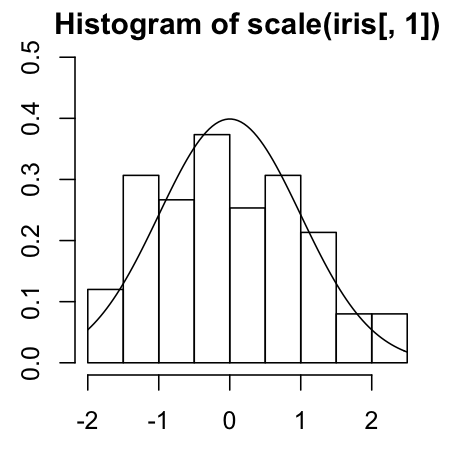
\includegraphics{figure/md-docx-fig1.png}
\caption{ヒストグラム}
\end{figure}

\section{最後に}\label{ux6700ux5f8cux306b}

Enjoy!!

\end{document}
